\documentclass[journal]{IEEEtran}
\usepackage[utf8]{inputenc} 
\usepackage[T1]{fontenc}
\usepackage[english]{babel}
\usepackage{listings}
\usepackage{textcomp}
\usepackage{placeins}
\usepackage{verbatim}
\usepackage{amssymb}
\usepackage[cmex10]{amsmath}
\usepackage{geometry}
\usepackage{listings}
\usepackage{graphicx}
\usepackage{enumerate}
\usepackage{caption}
\usepackage{cite}
\usepackage[colorlinks]{hyperref}
\usepackage{lipsum}
\usepackage{amsthm}
\usepackage{url}
\usepackage{array}
\usepackage{mdwmath}
\usepackage{mdwtab}
\usepackage{float}

\geometry{verbose,a4paper,tmargin=15mm,bmargin=22mm,lmargin=16mm,rmargin=16mm}

\title{Massively Parallelized Iris Recognition with CUDA}
\author{Platzer~Michael, Weber~Thomas, Zaruba~Florian}

\begin{document}

\IEEEcompsoctitleabstractindextext{%
\begin{abstract}
%\boldmath
Iris recognition is one of the most accurate biometric methods in use today. 
However, the two main approaches for implementing iris recognition algorithms are either on general purpose sequential processing systems, such as generic central processing units (CPUs) or on custom hardware field-programmable gate arrays (FPGAs).
Implementing iris recognition algorithms with CUDA represents a novel and low-cost alternative to systems solely based on CPUs or FPGAs. \cite{rakvic2009parallelizing}
\end{abstract}
% IEEEtran.cls defaults to using nonbold math in the Abstract.
% This preserves the distinction between vectors and scalars. However,
% if the journal you are submitting to favors bold math in the abstract,
% then you can use LaTeX's standard command \boldmath at the very start
% of the abstract to achieve this. Many IEEE journals frown on math
% in the abstract anyway. In particular, the Computer Society does
% not want either math or citations to appear in the abstract.

% Note that keywords are not normally used for peerreview papers.
\begin{IEEEkeywords}
iris recognition, CUDA, Hough transformation, Log-Gabor filter
\end{IEEEkeywords}}

\maketitle
\IEEEdisplaynotcompsoctitleabstractindextext
\section{Introduction}


\IEEEPARstart{I}{ris recognition} is nowadays one of the most favored biometric identification methods. It provides very high reliably regarding the unique identification of an individual. Quite recently India rolled out a large scale biometric identification program (including iris pattern) where at the time of this writing more than half the population are already enrolled into the program. \cite{daugmanspie}
\par Daugman, over the past years, has proposed several algorithms for iris recognition and had large impact on the techniques used for the Indian biometric identity cards as well. In one of his latest works he suggested some preprocessing steps in order to extract the iris from the image and subsequently generate a 2048 bit code from the phase information of several Gabor transformed iris images. Afterwards this IrisCode is matched against a database. \cite{daugman2004iris}
\par While the algorithm itself seems relatively sophisticated it performs some CPU-intensive operations like localizing the iris, unwrapping it and transforming it into time-frequency space with Gabor wavelets.
\par In the past two major approaches to that problem haven been proposed. On the one hand, there was an effort to implement the algorithm on general purpose multi-processor platforms as well as some specific digital circuits (FPGA implementation) specifically tailored to the needs of iris recognition.\cite{6417657}
\par Our approach on the other hand, tries to exploit the benefits of a general purpose graphics processing unit (GPGPU). In fact iris recognition involves many steps that are perfectly suitable for GPGPU since those algorithms are operating data parallel on images. In addition to the speed up the GPU gains in contrast to the CPU it is far more economically in terms of development and production costs than a custom circuit design on, for example, ASICs or even FPGAs.
\par In the present work we could demonstrate that an efficient implementation of an iris recognition algorithm on GPUs is indeed possible and brings significant performs gains towards a classical GPU approach. The implementation was tested with images from the CASIA Iris Image Database for Testing Version 1.0 (or IR-TestV1). \cite{ir-testv1}


\section{Related Work}
As mentioned before iris recognition plays a crucial role in biometric identification. For this reasons it has been improved tremendously over the past years. There were different approaches taken in the past to achieve maximum accuracy and retaining speed to a reasonable maximum.
\par As it comes to FPGA implementations in one case \cite{5487592} the system was implemented in a hardware/software codesign approach by using the Nios II soft-core. Other approaches exploited the additional advantage of re-programmable hardware devices by implementing custom hardware modules to additionally relief the (soft-)core in terms of computational resources. \cite{jimenez2006fpga, mohd2004fpga, hu2010iris}.
\par Current iris recognition algorithms can be grouped into three major types:
\begin{enumerate}
	\item phase-based methods \cite{daugman1993high}
	\item zero-crossing representation methods \cite{boles1998human}
	\item texture-analysis-based methods \cite{zhu2000biometric}
\end{enumerate}
\par Regardless of the matching technique used, the system has to reliably extract the iris from a given image. In 1987 the first relevant methodology was presented by Flom and Safir \cite{flom1987iris}. Some years later Daugman introduced an integrodifferntial operator to finding the inner and outer circle of the iris \cite{daugman1993high}. This approach still is relevant today and constitutes the basis of many functioning systems~\cite{proencca2006iris}.  Wildes proposed iris segmentation through a gradient-based binary edge-map construction followed by circular Hough transform. This is the most common approach today and can be found in several minor variants throughout the literature \cite{cui2004fast, huang2004new, kong2001accurate}.
\par In the paper at hand the implementation focuses on phase-based methods as proposed by Daugman \cite{daugman1993high} and preprocessing largely based on the gradient-based edge-map construction according to Borovicka~\cite{borovicka2003circle}. Our approach differs in the platform used for computation.
\par Daugman in addition proposed some interesting material about more robust feature extraction techniques such as Fourier-based methods allowing for off-axis gaze to be handled, statistical inferences methods for detecting and excluding eyelashes and more disciplined methods for detecting and faithfully modeling the iris inner and outer boundaries \cite{4305270}.
\section{Problem Description}
The objective of this application is the reliable and fast recognition of an iris from a given image, which is then compared against a potentially large database. The uniqueness of this approach is that most of the work involved is parallelized and given to a graphics processing unit (GPU) for fast parallel computation. The implementation at hand uses NVIDIA's parallel computatopm platform Compute Unified Device Architecture (CUDA)\footnote{\url{www.nvidia.com/object/cuda_home_new.html}}.
\par The task mainly consists of three steps: preprocessing and feature extraction, generation of a unique bit-sequence-representation of the iris and matching this sequence against a large dataset. At least the two former tasks are highly parallelizable and, as shown later, can largely profit from the computational power of GPUs.
\par The GPU implementation will pose an additional advantage on the task of iris recognition: With the emerging market of embedded graphics and general purpose processing unit platforms like the Tegra family from NVIDIA, our approach presents a low cost and low power alternative to traditional CPU or custom hardware implementations \cite{4483498}.
%\section{Background}

\section{System Overview}

This section presents our algorithm and techniques used for implementation of an iris recognition system. A general overview is depicted in Figure~\ref{fig:flow}.
\begin{figure}[ht]
	\centering
  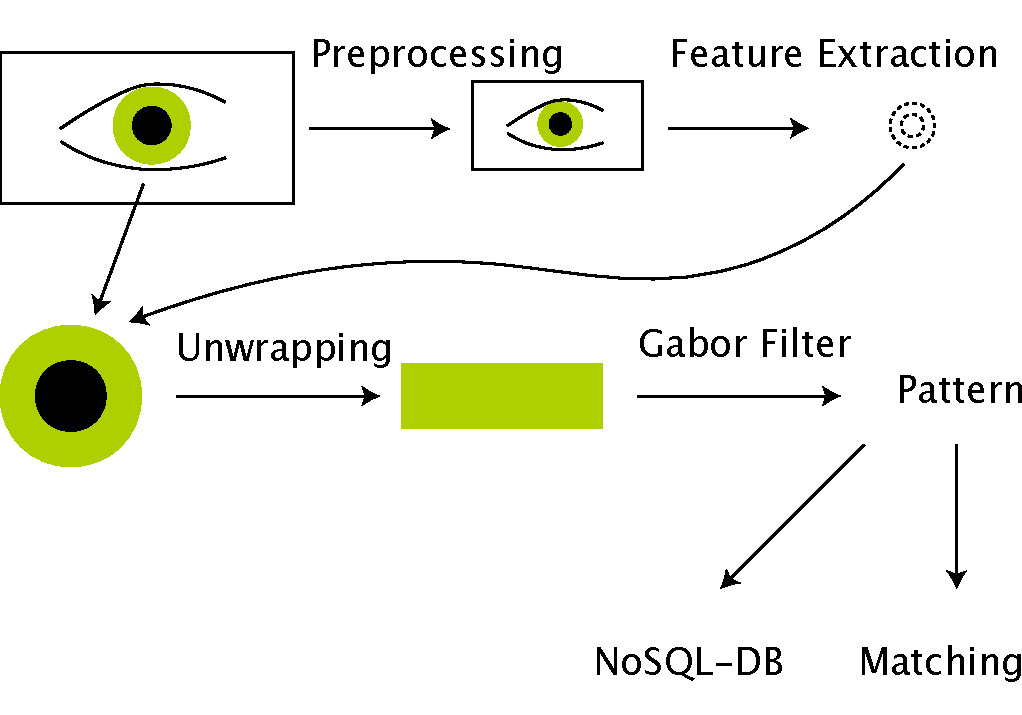
\includegraphics[width=0.45\textwidth]{iris/flow}
	\caption{Program flow of iris detection}
	\label{fig:flow}
\end{figure}
The main idea behind our approach is to perform most of the tasks at hand on a GPU. It turned out that the steps of preprocessing, feature extraction and most subtasks of unwrapping and Gabor filtering can be performed directly on the graphics unit therefore reducing the need on costly memory transfers between the host (CPU) and device (GPU). Furthermore multiple images can be scheduled to be processed simultaneously on the GPU (e.g. using multiple CUDA streams) thus making it even possible to analyze a real-time video-stream.
\subsection{Preprocessing}

The task of preprocessing involves various subtasks. The first one being a \emph{conversion from a (possibly) colored image to a grayscale} version. This reduces the amount of data necessary to handle the upcoming tasks. Color conversion is highly parallelizable since there is no dependency of individual pixels whatsoever. In most cases the conversion to greyscale does not influence the detection probability of the iris since most iris scanners in use, capture their images using infrared light in a darkened environment (closed glasses). A typical acquired image can be found in figure~\ref{fig:input}.
\begin{figure}[ht]
	\centering
  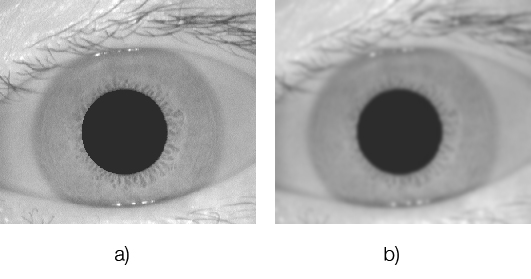
\includegraphics[width=0.49\textwidth]{iris/resized.jpg}
	\caption{a) Test image from the CASIA Iris Image Database for Testing Version 1.0~\cite{ir-testv1}. b) Image after Gaussian blur.}
	\label{fig:input}
\end{figure}
\par The second step consists of an \emph{image size reduction} of the greyscale input image to a fixed size. This, on the one hand, has the advantage of having an image that has at least its width a multiple of 32 (which turns out to be very efficient for processing on CUDA devices as it exploits the full warp size of a streaming multiprocessor subunit on the graphics chip). On the other hand, as will be discussed in the upcoming section, center detection is a relatively costly tasks in terms of processing power on the size of the image. A larger image does not improve center detection, on the contrary parameters of the tasks can be specifically tailored to the needs of a certain image and iris size (iris size in proportion to the overall image size). Resizing is accomplished by simply picking every other pixel that is needed for the targeted image size. It turned out that this approach is reasonably good suited for this purpose.
\par The third step involved is a \emph{noise reduction} of the image accomplished by a Gaussian blur. It turned out that resizing the image proposes an additional advantage: The Gaussian blur kernel depends largely on the image size. By constraining the image width one can set the filter kernel to a fixed size therefore making it possible to put the kernel into constant memory of the GPU. A second measure to improve computation speed was the fact that the Gaussian blur kernel has the property of being separable. This means that instead of performing one 2D convolution with the filter kernel one can perform two 1D convolutions therefore reducing the amount of arithmetic operations needed (instead of $n*m$ multiplications for each output pixel, where $n$ and $m$ are the width and height of the image only $n+m$ multiplications are needed)\cite{podlozhnyuk2007image}. Please see the appendix for a proof on the specified properties.
\par All three steps are highly profiting from the computational power and the GPU specific device architecture. The convolution in particular performs significantly faster than on traditional CPU systems. In addition to the above mentioned algorithmic details all loops are unrolled at compile time (since the size of the filter kernel is known) therefore reducing unnecessary jumps in the program flow and maximizing warp efficiency. In the present implementation all the memory access is coalescence in order to achieve maximum throughput.
\subsection{Feature Extraction}
Feature extraction is concerned with the task of identifying the iris in the image at hand. It basically accomplishes this task in two steps. First the eyes center is detected and afterwards, based on the center two contour lines are identified that form the iris boundaries.
\subsubsection{Center detection}
Regarding center detection the input image is convoluted with a Sobel filter. The Sobel filter consists of an 3x3 matrix for x (horizontal) and y (vertical) direction respectively \cite{sobel3x3}. The corresponding matrices can be seen in figure~\ref{fig:sobel}. 
\begin{figure}[ht]
\[
	G_x = \left(\begin{array}{ccc}
		-1 & 0 & 1 \\
		-2 & 0 & 2 \\
		-1 & 0 & 1 \\
	\end{array}\right) \quad G_y = \left(\begin{array}{ccc}
		-1 & -2 & -1 \\
		0 & 0 & 0 \\
		1 & 2 & 1 \\
	\end{array}\right)
\]
	\caption{Vertical and horizontal Sobel filter kernels.}
	\label{fig:sobel}
\end{figure} 
%% Maybe some images that give insights on the Hough transformation.
Basically, it is a discrete differentiation operator, computing an approximation of the gradient of the image intensity function. It performs poorly for high frequency variations in the image thus founding the reason why it is a good idea to perform a previous noise reduction step. The Sobel operator is separable as well thus making it easily possible to reuse the convolution function implemented for the Gaussian blur. In addition all advantages regarding the implementation of the Gaussian blur apply to the Sobel operation as well. In figure~\ref{sobel_hough} one can see the image after Sobel filtering. As it is clear from the example image the Sobel operator the operator produces an image that emphasizes the edges and transitions of the image on which it is applied.
\begin{figure}[ht]
	\centering
  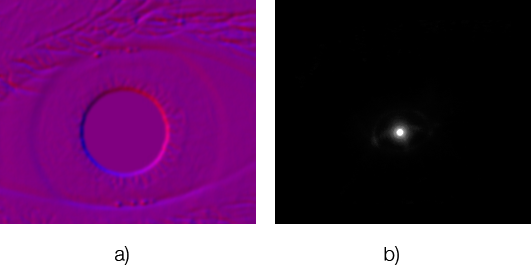
\includegraphics[width=0.49\textwidth]{iris/sobel_hough.png}
	\caption{a) Gradient map after Sobel opration (blue gradient component in x-direction and red gradient component in y-direction) b) heat map of center detection; center of gravity at (123, 133) pixels (at an overall image size of 320 pixels width and 280 pixels height).}
	\label{fig:sobel_hough}
\end{figure}
The next step involved is a \emph{Hough transform}. This transformation is a feature extraction technique mostly concerned with finding imperfect instances of certain parameterized curves \cite{shapiro2001computer}. In our cases we are interested in concentric circles and their respective center. The general idea is that perpendiculars to edge points of a circle cross in the center of the circle. Therefore, if we draw perpendicular lines to every edge point of our edge map, we should obtain bright 'hot spots' in the center of the circles.
\par In fact the implementation iterates through all possible $(x,y)$-coordinates and looks for radii of size $k$. In total running the Hough transform accumulates to a runtime of $O(x\cdot y \cdot k)$ which is, if we assume $x \geq y \geq y$, $O(x^2)$. For each possible center it looks for perpendicular lines around the given radius. If matching lines are found (e.g. the direction of the gradient points to the given center within a certain threshold of $[-\frac{\pi}{12},\frac{\pi}{12}]$) a local accumulator is incremented. By executing this algorithm we are left with a heat-map of potential centers (see figure~\ref{fig:sobel_hough}). In a next step we are looking for the \emph{average mean} of the heat-map which denotes a potential center of the iris. We are assuming that only one eye is present in the image and that it approximately takes up more than two thirds of the image. Those are crucial assumptions as it comes to parameter choices for the Hough transformation: By restricting the potential parameter space (radius size, margin areas, etc.) one can significantly speed up the transformation.
Furthermore we cube the values of individual radii in order to favor radii that perform reasonable good for most points on the radius over radii that are only accidentally well suited for some perpendicular lines.
\par Hough transformation highly benefits from a parallelized optimization. Potential centers are examined individually for each coordinate an can therefore be straight forwardly parallelized since there is no dependency between the dedicated coordinates whatsoever. For each radius one thread is launched and after the computation its result is stored in a shared variable structure and afterwards reduced (by addition) to a single value.
\begin{figure}[ht]
	\centering
  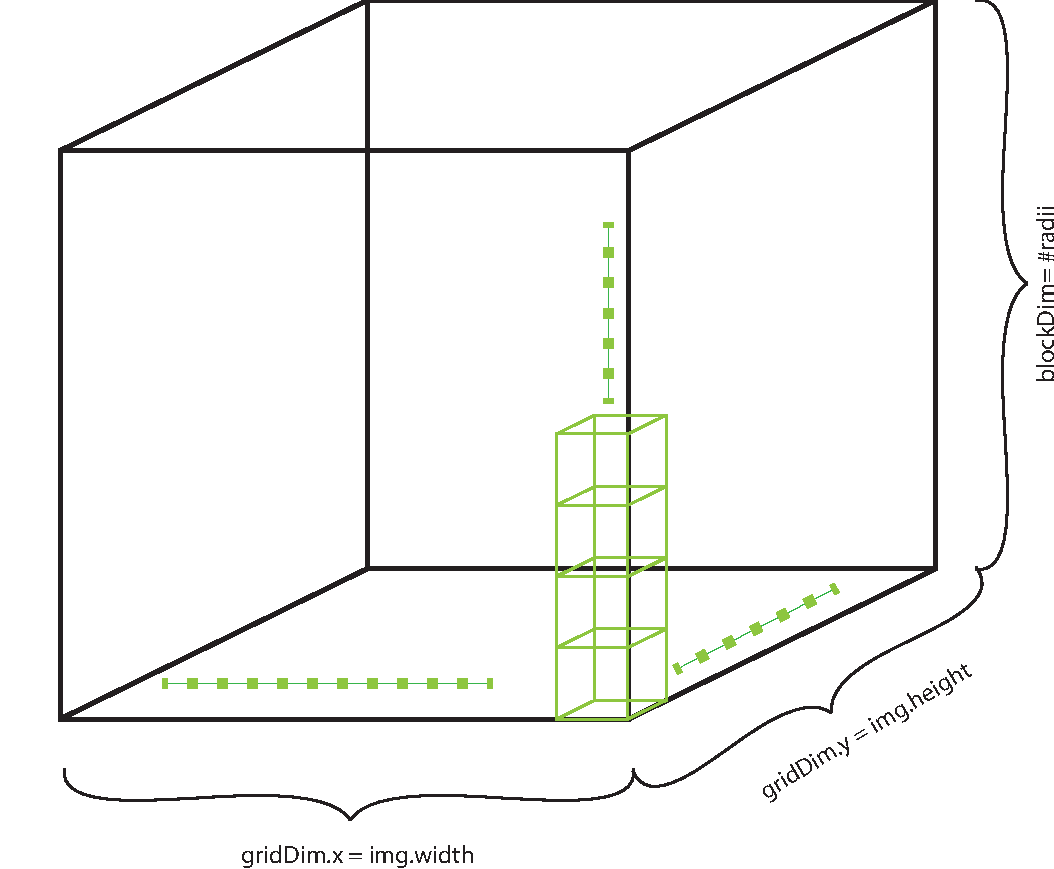
\includegraphics[width=0.49\textwidth]{iris/hough_impl}
	\caption{Thread structure of Hough transformation}
	\label{fig:hough_impl}
\end{figure}
\par  The thread structure can be examined in figure~\ref{fig:hough_impl}. Each block corresponds to a single thread. Blocks that are stacked denote threads of an individual block. Threads that share the block have a particular useful property namely, that they can access shared variables. Shared memory space performs significantly faster on thread access than global memory and is therefore often used for reductions of all kinds. We set our radius parameter space to a multiple of 32 to gain an additional advantage: Since CUDA Version 3.0 NVIDIA introduced a feature called warp shuffle functions. Essentially those features enable the GPU to pass different sorts of data between threads of a warp (a group of 32 threads that are implicitly synched by lock-step execution). This provided us with a toolset to exchange data (e.g. for a reduction) tremendously faster since there is no synchronization involved and data is directly stored in the cache blocks of each streaming multiprocessor respectively. This feature enabled us to reduce the vote values fore each radius on a warp basis which indeed gave a big speed up \cite{nvidiaparallel}.
\par As a last speed improvement the gradient map (in polar coordinates) resulting from the Sobel operation was stored in texture memory. Texture memory has the advantage that a specific pattern of localized memory access is cached and therefore retrieved faster. We where somehow lucky that this access pattern largely correlates to the usage by the Gough transformation (memory access should have 2D - spatial locality, e.g. its neighbors). On further advantage of the texture memory was the fact that an access needs not to be discretized (as it is the case for array access) and that an offset is linearly interpolated by the hardware in case of access outside the texture area or between to pixels or texels as they are called in case of texture memory. This has the advantage of limiting control flow structures for boundary detection and allows for coherent program flow of threads within the block (more accurately the warp).
\par The last step to obtain specific center coordinates involves finding the center of gravity. This is accomplished by averaging over the heat-map in x and y direction. This task can partly benefit from the optimization measures taken for the Hough transform. The task of additive reducing values directly applies to averaging as well. In addition a threshold value works as a low pass filter on the heat-map and discards values that are not significant for finding the center of gravity. 
\subsubsection{Radii detection}
The internals of radii detection and unwrapping are closely related. In a first pass we are enhancing the circular features of the iris' edges by computing the target angle (to be part of a circle) for each pixel $(x,y)$ and subtracting the actual angle.
\begin{align*}
	\varphi_t =& \tan^{-1}\left(\frac{y - y_{\text{center}}}{x - x_{\text{center}}}\right) \\
	\Delta \varphi =& \varphi_{(x,y)} - \varphi_t
\end{align*}
The angle difference is then fed to a standard Gaussian distribution which favors values close to zero.
\begin{align*}
	f = \exp\left(-\frac{(\Delta \varphi)^2}{\sigma^2}\right)
\end{align*}
Subsequently this factor is multiplied with the Euclidean norm of the gradient map at position $(x,y)$. An example of such an enhancement is displayed in figure~\ref{fig:sobel_norm}.
\begin{figure}[ht]
	\centering
  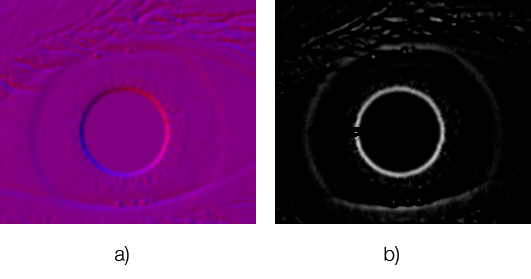
\includegraphics[width=0.49\textwidth]{iris/sobel_norm.png}
	\caption{a) Gradient map after Sobel operation b) Normalized gradient map, curves that are not concentric to the computed center are suppressed}
	\label{fig:sobel_norm}
\end{figure}
For further processing, the iris is projecting from a circular representation to a quadratic image e.g. it is unrolled with regard to its previously calculated center coordinates. In this first step where the exact iris borders are still unknown it is unrolled with respect to the greatest possible radius. The unrolled iris from figure~\ref{fig:sobel_norm} can be seen in figure~\ref{fig:unrolled}. 

\begin{figure}[ht]
	\centering
  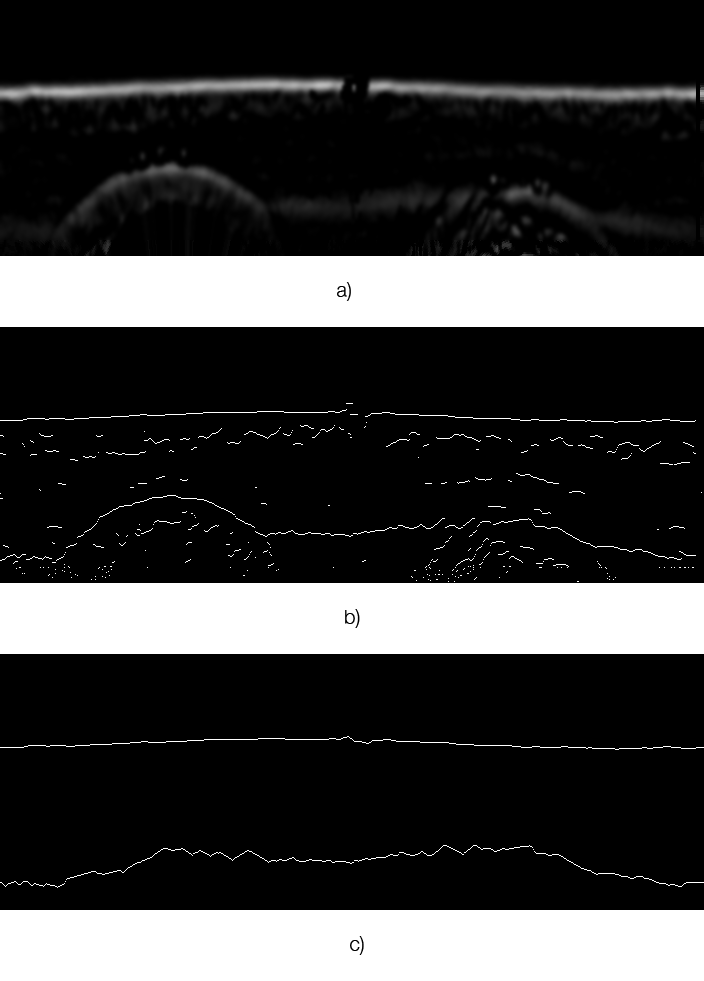
\includegraphics[width=0.49\textwidth]{iris/unrolled.png}
	\caption{a) unrolled and blurred iris b) local maxima are set to the highest value c) traces of iris boundaries}
	\label{fig:unrolled}
\end{figure}

The unrolling algorithm directly interacts with the gradient map stored in the texture memory which was used in the previously performed Hough transformation. This has the advantage that memory access to 'unspecified' memory locations is transparently handled and linearly interpolated. This makes a lot of sense when considering an unroll operation: Since samples taken from regions close to the center are over-sampled whereas iris regions which are further away from the center tend to be under-sampled. This task is easily parallelizeable by launching kernels for each pixel in the target image (the image size of the unrolled iris is fixed). Unrolling corresponds to a \emph{transformation to dimensionless polar coordinates} (where the image width corresponds to the angle $\varphi \in [0, 2\pi]$ whereas the height corresponds to the radius $r \in [0, 1]$).
% why gaussian blur
\par It is quite unpractical for decisions on iris boundaries to work with blurred contour lines, ergo we want to reduce the contour lines to sharp decision boundaries. This is accomplished by searching for local maxima and setting these values to a easily distinguishable value. The output of this step can be seen in figure~\ref{fig:unrolled} b). Basically the algorithm compares each value with the value of its predecessor and successor. If the current value is greater than the other two values it implies that it is a local maximum. The algorithm additionally uses a certain threshold to avoid unintentionally considering noise as an extrema. 
\par The last step that remains for the task of radii detection is to decide for the correct contour lines of the iris. This is done with an Bayesian decision approach that assigns costs to each individual trace. Two of the traces with the least costs are then chosen as possible iris boundaries. The image is traversed from left to right. For each pixel in the first column a corresponding pixel in the next 60 columns are searched. The costs for the route increase proportional to the distance of the next pixels to the estimated route (e.g. a straight line). The search space has a triangular shape which implies that only pixels within this window are considered for potential successors of the line segment.
\begin{figure}[ht]
	\centering
  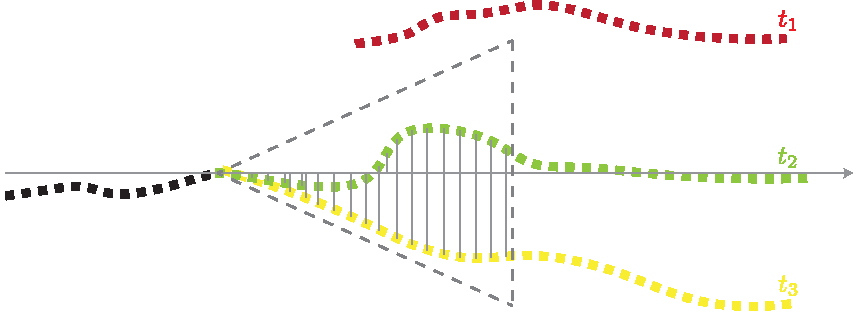
\includegraphics[width=0.49\textwidth]{iris/trace}
	\caption{The tracing process is depicted for 3 different traces $t_1$, $t_2$ and $t_3$. While $t_1$ is not recognized $t_2$ has a lower cost function assigned than $t_3$.}
	\label{fig:trace}
\end{figure}
One such an example of line tracing can be seen in figure~\ref{fig:trace}. The first trace ($t_1$) is not recognized since it lays outside the decision window. This allows for successfully suppressing artifacts that can accidentally occur within the iris. The second trace $t_2$ has a lower cost function than $t_2$ since it progresses closer to the optimal line segment.
\par The resulting traces and the center are then calculated for the original image by multiplication with the image compression factor. The original image and the traces shown in the original image form a cut mask (see figure~\ref{fig:iris_cut_mask}).
\begin{figure}[h]
	\centering
  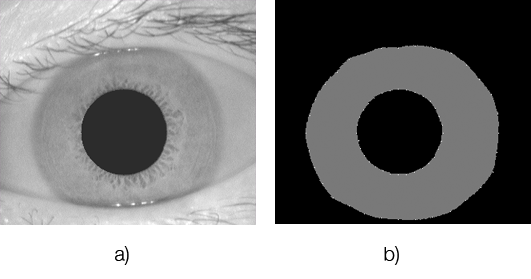
\includegraphics[width=0.49\textwidth]{iris/iris_cut_mask.png}
	\caption{a) original iris image b) generated cut mask}
	\label{fig:iris_cut_mask}
\end{figure}

\subsection{Unrolling}
The same unrolling operation used in the previous step is used for unrolling the final iris from the original image given the cut mask. Such an unrolled iris can be seen in figure~\ref{fig:unrolled_iris} a). As one may notice: The iris unrolling is imperfect due to various reasons, one being partial coverage of the iris by the eyelid. Some algorithms account for that imperfection by ignoring the covered part in the later step of feature generation and pattern matching (for example Daugman \cite{4305270}). In the current implementation we do not account for that. 
\begin{figure}[ht]
	\centering
  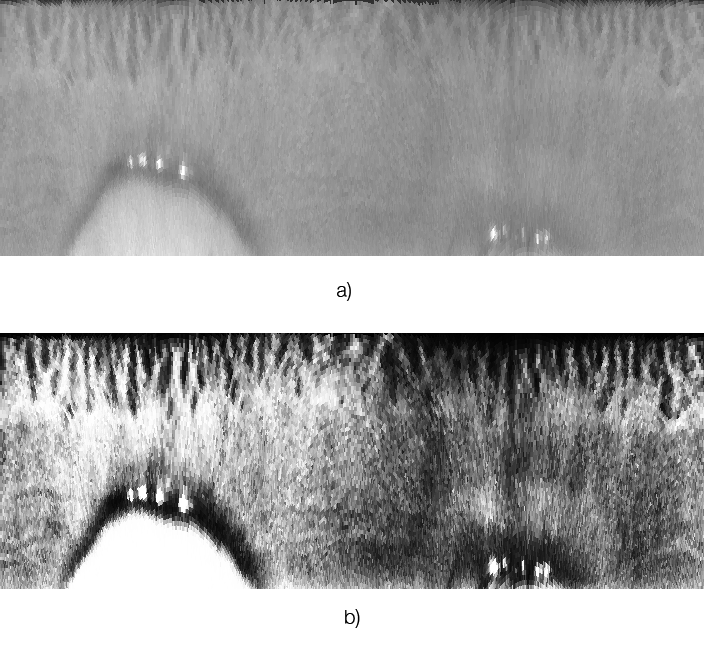
\includegraphics[width=0.49\textwidth]{iris/iris_unrolled.png}
	\caption{a) original cropped iris pattern b) equalized iris pattern - single features are more easily detectable}
	\label{fig:unrolled_iris}
\end{figure}
\par It turns out that the spectrum used for representation of the iris is rather narrow. A histogram for the example image is depicted in figure~\ref{fig:histogram}. In order to enhance the performance in the later step of pattern matching we are equalizing the image over the whole grey space of 256 bit in the current implementation. This approach usual increases the global contrast of many images.
\begin{figure}[h]
	\centering
  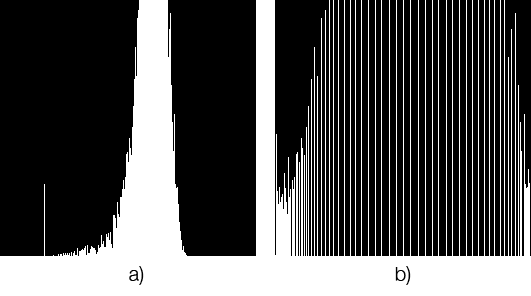
\includegraphics[width=0.49\textwidth]{iris/iris_histo.png}
	\caption{a) Histogram of the unrolled iris image. 256 grey values on the x-axis and overall count of the respective values on the y-axis b) Histogram of the equalized iris image}
	\label{fig:histogram}
\end{figure}
The process of histogram equalization generally distinguishes two concepts of thinking. Either the processes is viewed as a image change or as a palette change. While in the first individual pixels are immediately substituted in the latter the palette is changed. In our implementation first the palette is substituted and afterwards according to the changed palette the image is substituted.
A cumulative distribution function (cdf) is generated according to the previously generated histogram.
\[
	cdf_x(i) = \sum \limits_{j=0}^{i} p_x(j) \qquad i \in [0, 255]
\]
And the new palette is then generated by:
\[
	pal(i) = cdf_x(i) \cdot 255  \qquad i \in [0, 255]
\]
The corresponding generated histogram and image are depicted in figure~\ref{fig:unrolled_iris} b) and figure~\ref{fig:histogram} b) respectively.
\subsection{Pattern Generation}
The next part deals with the generation of a pattern (or feature vector) that uniquely determines the iris. The feature vector should have the properties to be as small as possible (in terms of byte size) in order to be stored, retrieved and matched as fast as possible from a potentially large dataset. In addition the feature vector should be largely invariant to rotations, dilatations and images properties like brightness, hue and contrast. Various approaches to this problem are persecuted in the literature. We decided our implementation in favor of a Log Gabor filter and subsequent calculation of an average absolute deviation of gray values (our implementation is mostly based on the ideas of Seif et al.\cite{seif2003iris}). 
\subsubsection{Log Gabor filtering}
The Gabor filter is able to simultaneously analyze the space and frequency characteristics of a given signal. There exist numerous transformations (variations of the short-time Fourier transform) that share that same characteristic however, the Gabor filter achieves optimal in terms of the space-frequency tradeoff \cite{gabor1946theory}. The Log Gabor filter in particular is one improvement of the Gabor filter in the way that fits the statistics of natural images. In fact there is some evidence that Log Gabor filtering performs similar to how the human visual system processes information \cite{daugman1985uncertainty}. In addition the Log Gabor filter has a zero DC component, hence the response does not depend on the mean value of the signal. The difference in the frequency responses can be seen in figure~\ref{fig:frequency_response}. As shown by the plot the Gabor filter over-represents low frequencies. The third frequency response is the same as the second but instead of a linear frequency axis a logarithmic axis is used. When represented in this manner the response becomes a Gaussian bell formed curve.   
\begin{figure}[t]
	\centering
  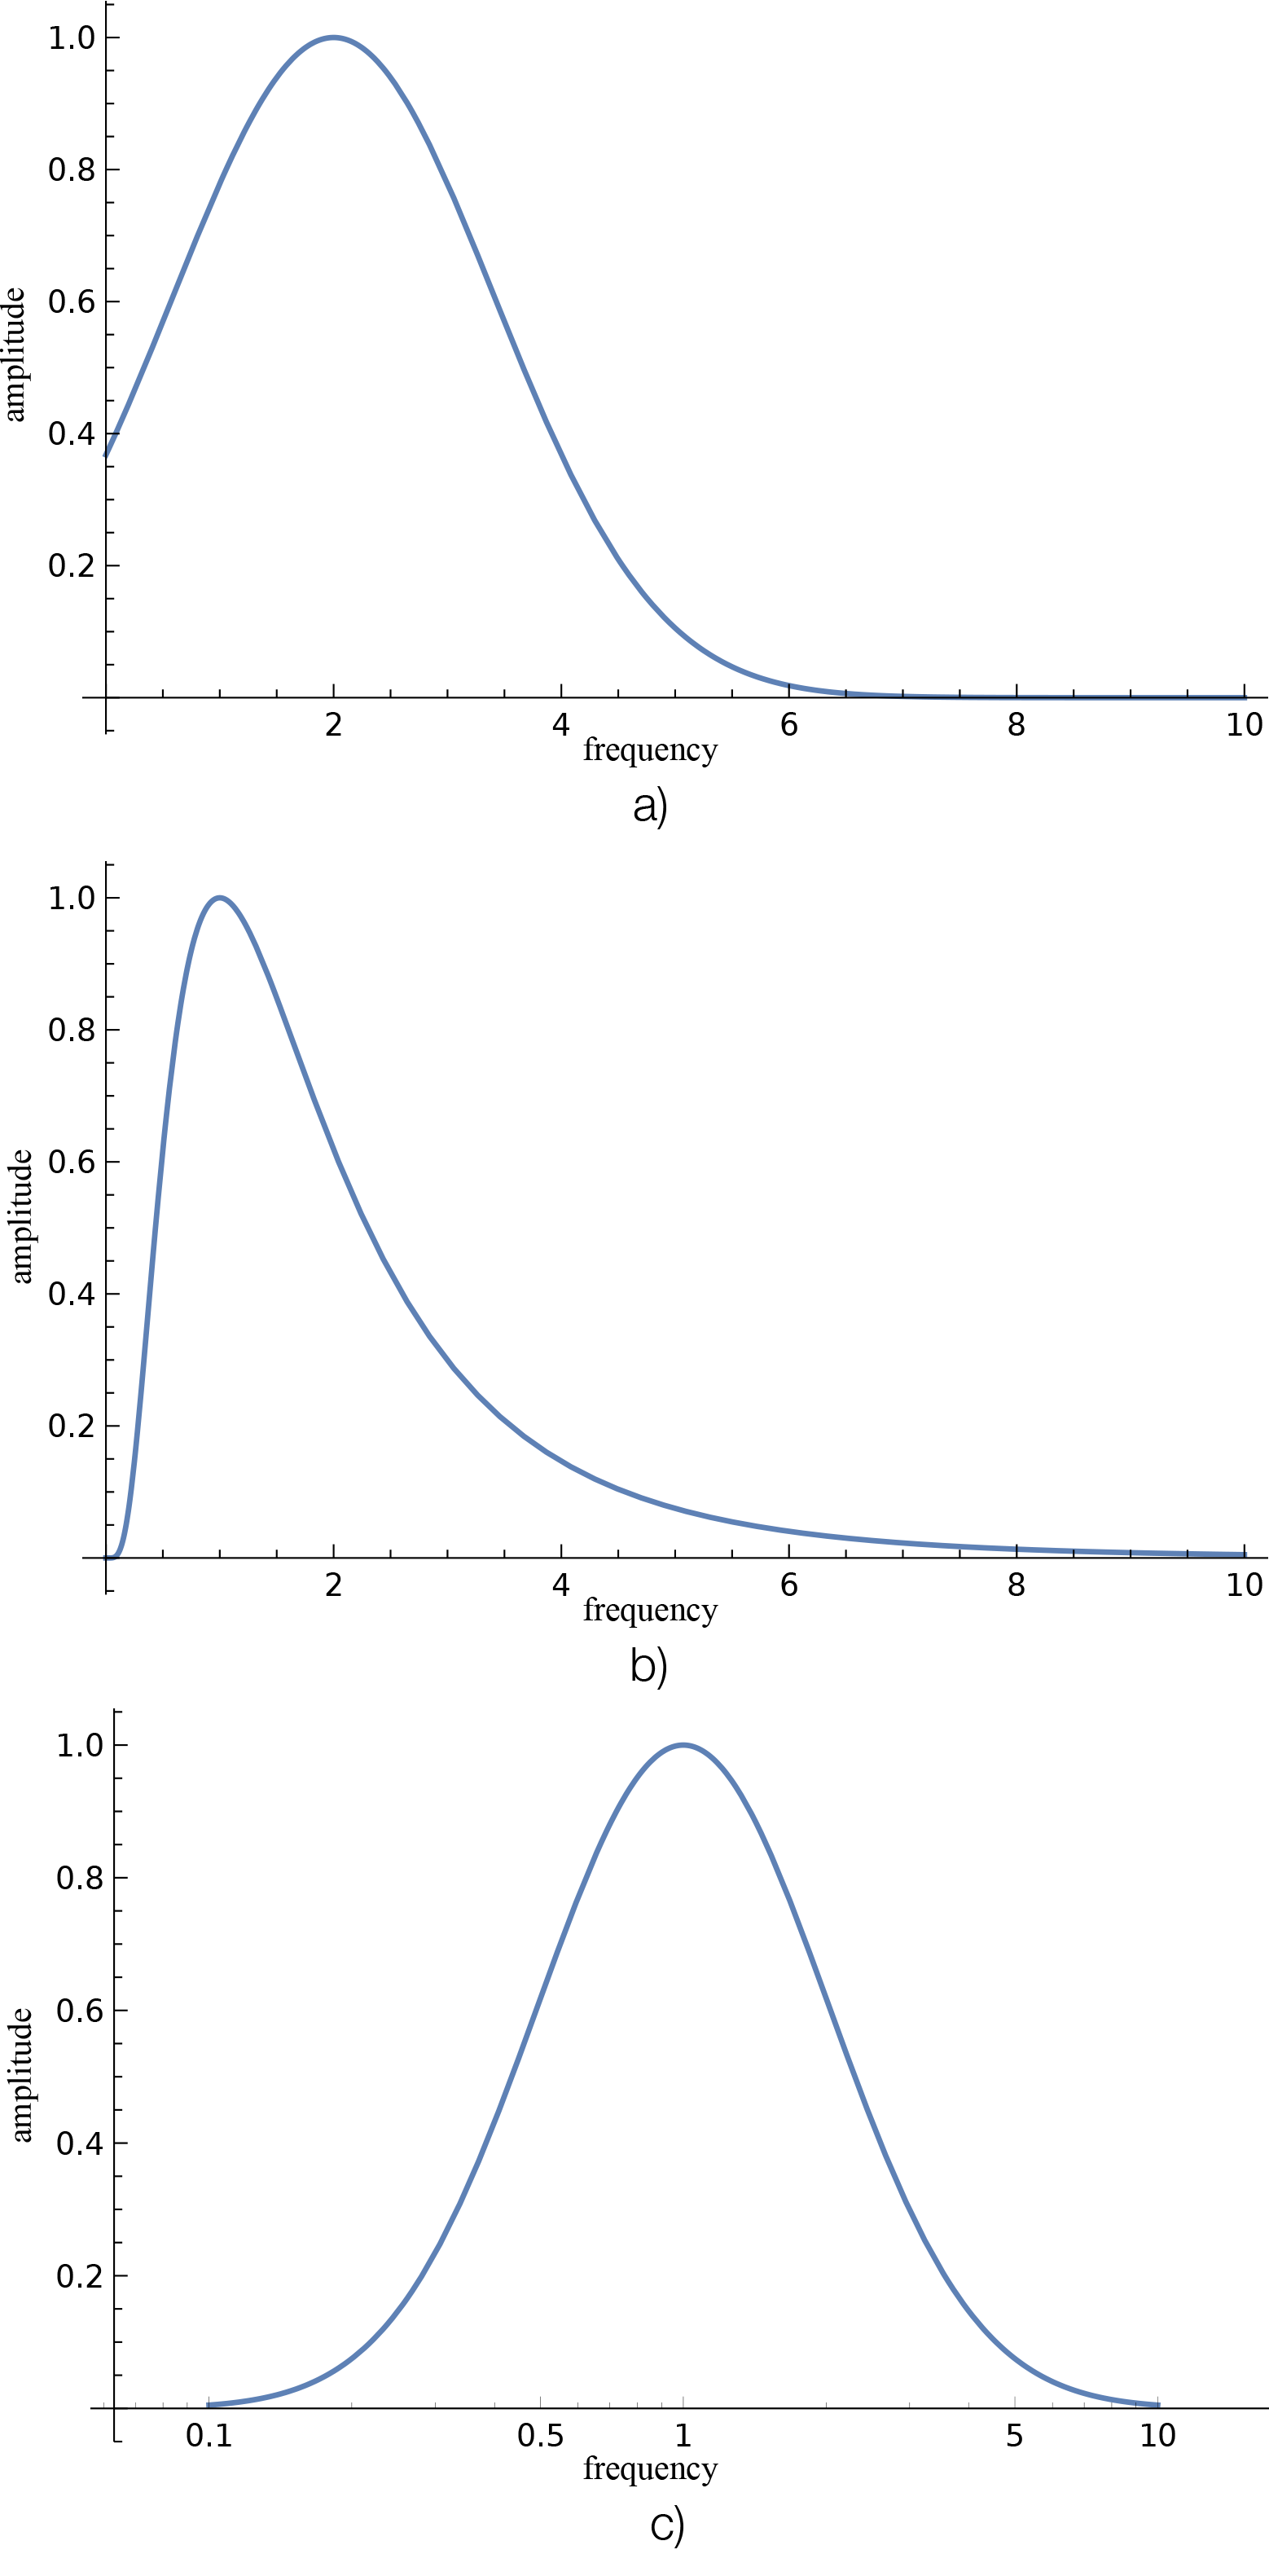
\includegraphics[width=0.49\textwidth]{iris/freq_response_gabor.png}
	\caption{frequency response of  a) Gabor filter b) Log-Gabor filter c) Log-Gabor filter depicted with a logarithmic frequency axis}
	\label{fig:frequency_response}
\end{figure}


The one dimensional Log Gabor function has the frequency response of:
\[
	G(f) = \exp\left( \frac{-(\log(f/f_0))^2}{2(\log(\sigma/f_0))^2}\right)
\]
where $f_0$ and $\sigma$ are the parameters of the filter, $f_0$ will determine the center frequency of the filter. Because of the zero at the DC value, it is not possible to derive a closed form expression in the time/space domain, therefore the filter is designed in the frequency domain and transformed to the time/space domain in a subsequent step.
\par So far we only considered one dimensional Log Gabor filters. For the task of image processing it is useful to take a two dimensional version of the Log Gabor filter into consideration. For this purpose the transfer function is multiplied with a second Gaussian that additionally restricts the window in the second dimension and therefore imposing a direction on the filter. A representation of such a two dimensional filter in the time/space domain is depicted in figure~\ref{fig:2Dloggabor}. One can identify the Log Gabor function on the x-axis while in contrast on the y-axis a simple Gaussian function contributes to the plane. The z-axis shows the real part of the filter. 

%Wieso 45 grad??
\par For this particular implementation we are only considering two directions for reasons explained further below. By varying frequency and orientation parameters it is possible to generate a filter bank that enhances different features of the iris. The creation of the filter bank and therefore the choices of the parameters is somehow unique to the application. No general approach is known for this task. 

\begin{figure}[H]
\centering
  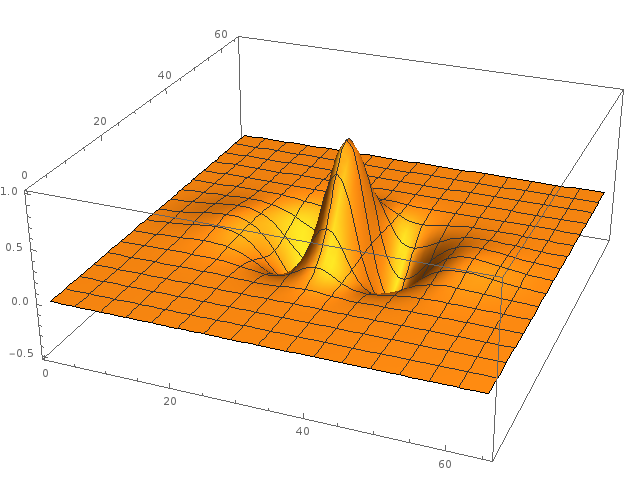
\includegraphics[width=0.39\textwidth]{iris/log_gabor_2d.png}
	\caption{3D representation of a Log Gabor filter's real part in the time domain}
	\label{fig:2Dloggabor}
\end{figure}

A small subset of the filter bank used in the implementation at hand is shown in figure~\ref{fig:filter_bank}. One can spot the different filter directions and frequencies in use. The bright parts of the filter correspond to large (amplifying) values while the dark part is essentially suppressing parts of the convolved image.


\begin{figure}[t]
	\centering
  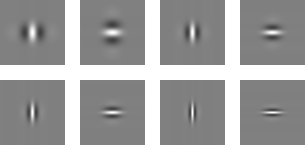
\includegraphics[width=0.49\textwidth]{iris/2d_log_gabor_filter.png}
	\caption{Small subset of the Log Gabor filter bank used}
	\label{fig:filter_bank}
\end{figure}

\begin{figure}[t]
	\centering
  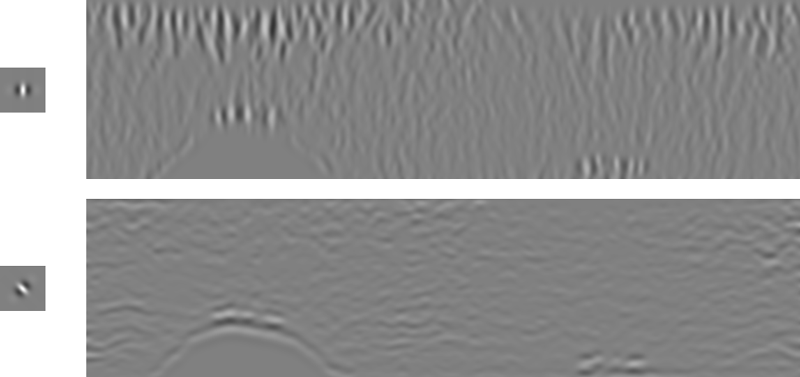
\includegraphics[width=0.49\textwidth]{iris/pattern_gen.png}
	\caption{}
	\label{}
\end{figure}


\subsubsection{Feature Vector Generation}
\[
D = \frac{1}{N\cdot M} \sum \limits_{x=0}^N \sum \limits_{y=0}^M |f(x,y) - \mu|
\]

\subsection{Pattern Matching}
After performing the Gabor transformation we aimed to take its output to do the pattern matching of two iris images. Thus each iris image is transformed into a 256 long character string (also called “iris matrix”) a humongous amount of data has to be stored and matched. This procedure cannot be done with common SQL database engines because they are not able to perform read/write commands to thousands of big sets of data within few  microseconds. As a consequence to the matter of this fact the conventional SQL approach has to be dropped and noSQL databases, which are explicitly designed for such purposes, were chosen. The disadvantage of such noSQL databases (e.g. mongoDB, OrientDB, CouchDB, Lotus Notes) is the weak data consistency which can be disregarded in the context of iris recognition concerning the relation of one or two bytes in relation to 256 bytes. The database “mongoDB” is used in this implementation.
\par To search for an iris in the database it is essential to choose an remarkable and unique vector out of the searched iris matrix. This vector, that we also call “feature vector”, contains the most significant samples out of a iris matrix. The feature vector can be gained by selecting a window of samples out of the matrix (see Figure~\ref{pic:picture1}) which leaves enough space between the outer circle of the iris to avoid image errors caused by eyelashes and eyelids, especially in case of small eyes and eyes with the epicanthic fold. Thus the unrolling generates multiple redundant vector data of the inner iris image, the possibility for a match with the same generated pattern in a iris matrix from a different eye is higher. Therefore, a feature vector should not contain much data of the inner part from the iris.
\par With the generated feature vector it is now possible to search for matching iris matrices in the database. This is done by substring comparison. All found candidates are full bit wise compared to calculate the hamming distance between the sample matrix and the matrix from the database. To avoid false positives a threshold value for the hamming distance is used. In case of multiple matches, the iris with the smallest hamming distance is chosen.

\section{Implementation}

\lipsum[3]

\section{Results}
\lipsum[3]

\section{Conclusion}
\lipsum[3]

 
\bibliographystyle{plain}
\bibliography{references} 

\begin{appendix}
	\begin{proof}
		By definition of the 2D discrete convolution:
		\[
			y[m,n] = x[m,n]*g[m,n] = \sum \limits_{i=-\infty}^{\infty} \sum \limits_{j=-\infty}^{\infty} x[i, j]\cdot g[m-i, n -j]
		\]
		By commutativity of the convolution
		\[
			y[m,n] = g[m,n]* x[m,n]= \sum \limits_{i=-\infty}^{\infty} \sum \limits_{j=-\infty}^{\infty} g[i, j]\cdot x[m-i, n -j]
		\]
		and the seperability property of $g[i, j] = g'[i] \cdot g''[j]$ we acquire:
		\begin{align*}
			y[m,n] &=\sum \limits_{i=-\infty}^{\infty} \sum \limits_{j=-\infty}^{\infty} g'[i] \cdot g''[j] \cdot x[m-i, n -j] = \\
			&=\sum \limits_{i=-\infty}^{\infty} g'[i] \cdot \sum \limits_{j=-\infty}^{\infty}  g''[j] \cdot x[m-i, n -j] = \\
			&=\sum \limits_{i=-\infty}^{\infty} g'[i] \cdot \left(\sum \limits_{j=-\infty}^{\infty}  g''[j] \cdot x[m-i, n -j] \right) \\
		\end{align*}
		By plugging in the definition of a 1D discrete convolution $y[n] = x[n]*g[n] = \sum \limits_{i=-\infty}^{\infty} x[n]*g[n-i]$, we get:
		\begin{align*}
			y[m, n] &= (g'[m] \cdot g''[n])*x[m, n] = g'[m]*(g''[n]*x[m,n]) \\
			&=  g''[n]*(g'[m]*x[m,n])
		\end{align*}
	\end{proof}
	\begin{proof}
		We want to show the seperabilty of the Gaussian filter kernel. Seperability would mean that
		\[
		G(x,y) = G(x)\cdot G(y)
		\]
		The 2D $G(x,y)$ and 1D version $G(x)$  of the Gaussian filter kernel are defined as follows:
		\begin{align*}
			G(x,y) &= \frac{1}{2\pi \sigma^2}e^{\frac{x^2+y^2}{2\sigma^2}} \\
			G(x) &= \frac{1}{\sqrt{2\pi} \sigma}e^{\frac{x^2}{2\sigma^2}}
		\end{align*}
		Obviously by plugging in the definitions we obtain
		\begin{align*}
			G(x)\cdot G(y) &= \frac{1}{\sqrt{2\pi} \sigma}e^{\frac{x^2}{2\sigma^2}} \cdot \frac{1}{\sqrt{2\pi} \sigma}e^{\frac{y^2}{2\sigma^2}} = \\
			&= \frac{1}{2\pi \sigma^2}e^{\frac{x^2+y^2}{2\sigma^2}}
		\end{align*}

	\end{proof}
	\begin{proof}
		We want to show the seperability of the Sobel filter.
		\[
			G_x  = \left( \begin{array}{ccc}
			-1 & 0 & 1
			\end{array}\right) \cdot  \left(\begin{array}{c}
			1 \\
			2 \\
			1
			\end{array}\right) = \left(\begin{array}{ccc}
				-1 & 0 & 1 \\
				-2 & 0 & 2 \\
				-1 & 0 & 1 
			\end{array}\right)
		\]
		\[
			\quad G_y = \left( \begin{array}{ccc}
			1 & 2 & 1
			\end{array}\right) \cdot  \left(\begin{array}{c}
			-1 \\
			0 \\
			1
			\end{array}\right)
			= \left(\begin{array}{ccc}
				-1 & -2 & -1 \\
				0 & 0 & 0 \\
				1 & 2 & 1 \\
			\end{array}\right)
		\]
	\end{proof}
\end{appendix}
\end{document}
